This chapter provides the theory behind Apache Flink and Kafka Streams, key concepts,
illustrative examples, and main challenges.
A reader should be able to understand the context and why such frameworks are needed.
Both frameworks are based on principles of distributed systems design,
which are all covered in the context of a given problem.

%\section{Simple use case}\label{subsec:why-framework-is-needed}
%Let's define a simple task that is given by a business.
%For example,  the business wants to know what songs get more streams in different countries.
%A straightforward solution is the code below.

\section{Scalability Problems}\label{subsec:simple-pip}
Let's define a simple task that is given by a business.
For example, the business wants to know what songs get more streams in different countries.
A straightforward solution is the code below \ref{lst:chart_list}.

\small
\begin{lstlisting}[label={lst:chart_list}]
    top_charts = db.select("top_charts")
    ordered_bands = top_charts
        .group_by(chart -> chart.country)
        .agreggate_by(chart -> chart.streams)
        .order_by(chart -> chart.streams)
        .map(chart -> {chart.streams, chart.song, chart.country})
\end{lstlisting}
\normalsize

\begin{figure}[H]
    \centering
    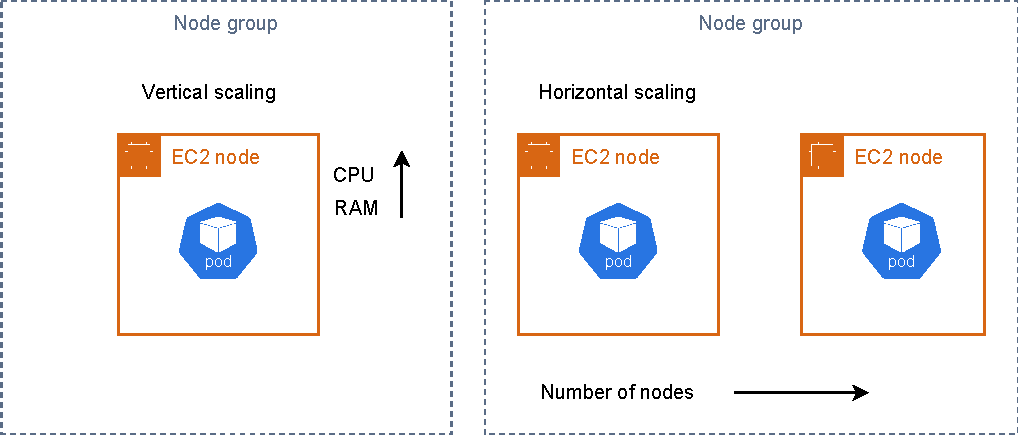
\includegraphics[width=1\textwidth]{figures/vertical-horizontal-scaling}
    \caption{\textit{Example of vertical and horizontal scaling where vertical is about using more powerful node
    and horizontal about adding more nodes.}}
    \label{fig:vert-hor-scal}
\end{figure}

The first straightforward solution is to use a more advanced node \cite{aws_node_types} with more CPU, RAM, and Cores.
Such a solution works until there's no such powerful node that can process high volumes of data.
Even if such a node still exists, it might lead to processing downtime if the node is down for some reason.
Adding additional resources such as CPU and RAM refers to vertical scaling that scales less than horizontal scaling \cite{vertical_horizontal_scalling_1}.
Example on Figure \ref{fig:vert-hor-scal}.

Even having a scaling setup, big data processing is not that straightforward to scale without having
in an efficient distributed processing model.
These models are MapReduce \cite{map_reduce_google, map_reduce_2, map_reduce_3} and DAG \cite{flink_dag, kafka_streams_topology}.
There are open-source solutions which implement one of model and successfully being used in industry \cite{flinkPoweredBy, netflixStreamingSQL}.
Moreover, they provide an api which
look almost the same as map, filter, reduce functions.

Here are key points about frameworks for data pipelines such as Apache Flink, Kafka Streams and
Apache Flink, that use complex DAG model under the hood.

\begin{description}
    \item[Scalablity] These frameworks are designed to be scalable by default.
    The main difference in scalability is that frameworks use models such as
    MapReduce, DAG.
    It means that frameworks know how to be scalable under the hood,
    using multiple nodes.
    Framework knows how to distribute sub-problems across multiple parallel workers
    and combines multiple sub-results into a single result.
    Execution performance is achieved by having multiple
    parallel workers that shuffle a data stream by key and distribute a load between each other.
    \item[Fault Tolerance] Frameworks are designed to be tolerant to faults.
    The Common approach is replication, rebalancing, and a state reprocessing after recovery.
    However, they're different depending on a framework.
    For example, Kafka Streams is based on changelog topics \cite{confluentKafkaStreamsFaultTolerance},
    Apache Spark uses RDD or resident distributed datasets \cite{Zaharia2012RDD} , Apache Flink
    uses distributed snapshots, the algorithm is well covered in \cite{flinkCheckpoints}.
    \item[Kubernets operator] Modern frameworks are designed to be run in the Kubernetes environment.
    Kubernetes operators are used to manage such complex deployments in production \cite{flink_kubernetes_operator}.
    \item [Built-in integrations] For example, it can be machine learning pipelines, external data sources,
    graph processing algorithms \cite{JMLR:v17:15-237, flink_ml_reseach, flink_ml}.
\end{description}

%\subsection{Simple example with Apache Spark}\label{subsec:simple-spark}
%
%With a framework the pipeline looks the same, but with having all these features
%provided in the list above.
%
%\begin{lstlisting}[label={lst:spark}]
%spark = SparkSession.builder
%    .appName("Country Musical Streams")
%    .getOrCreate()
%
%df = spark.read.csv(data_path)
%result = df.groupBy("country")
%    .agg(sum("streams").alias("total_streams"))
%    .order_by(chart -> chart.streams)
%    .map(chart -> {chart.total_streams, chart.song, chart.country})
%
%\end{lstlisting}
%
%Frameworks allow to reuse already existing pipelines and make relly reliable
%and scalable solution.
%This is just a small example to imagine how it's used and why.
%The next chapter goes to a technical details more deeply.


\section{Stream Processing}\label{sec:-concepts}
Stream processing is a concept that is dedicated to systems that need to process an infinite
message or event, often called an unbounded dataset \cite{Dataflow2015}.

A stream has a quite broad meaning, it often gets referred to
stdin and stdout of Unix programming languages \cite{kleppmann2017}.
For some developers, stream could mean file stream API and
for an average person it would mean video content stream, for example
on YouTube or on Twitch.
In this case study, the stream refers to infinite dataset that represents
a infinite dataset.

\begin{figure}[H]
    \centering
    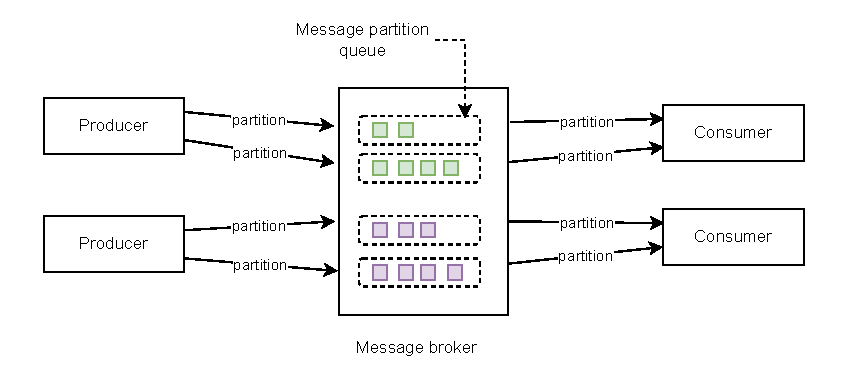
\includegraphics[width=1\textwidth]{figures/producer-consumer}
    \caption{\textit{This diagram illustrates a message queue system optimized for handling unbounded datasets.
    Each partition has its own queue.}}
    \label{fig:producer-consumer}
\end{figure}


%It is important to know that a difference between these patterns might be tricky,
%lots of details depend on a certain pattern implementation.
%For example, Apache Kafka uses producer/consumer, but Apache Pulsar uses published/subscriber.
%Both can be used for a data streaming, it is important to figure out what does a business
%actually want, before developing a solution.

%\subsection{DAG}\label{subsec:dataflow-graph}
%This is the core part which confuses lots of developers who are not familiar
%with data processing frameworks.
%In the previous chapter, two scripts with a data pipeline were provided, where
%one uses a standard language api and another is written with Apache Spark.
%Such frameworks like Apache Spark, Apache Flink and Kafka Streams actually
%use dataflow graph model under the hood, to achieve a high performance and parallelism.
%Just implementations might be slightly different.
%
%Since some developer wind parallelism quite challenging to
%understand, not just a parallelism itself by rather a model
%its evolution, how did the data systems get to this moment.
%It's actually an evolution log research which has taken decades and
%it's quite complicated to imagine what's going to be next evolution
%in data streaming systems.
%
%\begin{description}
%    \item[Dataflow Architectures] In 70s, researchers were looking for new approach in
%    designing parallel computing systems.
%    These prototypes represented computations in directed graphs,
%    where nodes were operations and edges indicated data dependencies.
%    These prototypes allowed to achieve an asynchronous and fine-grained parallelism,
%    which was a departure from the conventional von Neumann architecture.
%    Some notable dataflow machines from this era include the Manchester Dataflow Machine,
%    MIT's VAL, and the Japanese ETL-Mark-III.
%    \item[Dataflow Programming Languages] Next step was between 70-80s.
%    First dataflow programming languages were developed to handle parallel programming challenges.
%    These languages, such as Id, SISAL, and Lucid, used dataflow principles
%    to express parallelism explicitly and manage dependencies between operations.
%    This allowed developers to focus on application business logic rather on parallelism
%    while the runtime system took care of scheduling and synchronization.
%    Obviously there were that advanced as modern programming languages as java or C++, but it
%    was a significant progress.
%    \item[Dataflow Models for Parallel Processing] Further research on dataflow models moved
%    focus from hardware architectures to software-based dataflow models,
%    which enabled a higher level of abstraction and portability.
%    Some of these models, like the Bulk Synchronous Parallel (BSP) and LogP,
%    influenced the design of parallel programming libraries and frameworks, such as MPI and PVM.
%    Progress in new languages programming languages such C/C++ a more advanced hardware did
%    a big step to focus more on software models.
%    \item[Dataflow Models for Data Processing] This is a modern era of dataflow models in distributed computing.
%    Dataflow models gained renewed interest as a way to represent and reason about data processing pipelines.
%    Systems like Google's MapReduce, Apache Hadoop, and Apache Spark adopted dataflow
%    concepts to enable large-scale data processing in distributed environments.
%    MapReduce gave a huge step forward for modern data processing frameworks, however,
%    MapReduce is getting less popular due popularity of Apache Flink and Kafka Steams which
%    adopted MapReduce and dataflow model for a real time stream processing.
%    At the moment dataflow graphs as a core component for modeling real-time data processing pipelines,
%    which provides a great performance in an ease in use by provide a high-level api.
%\end{description}
%
%This brief history gives a high-level overview about moder data processing system to
%understand a main difference between running a simple script or running on top of
%data processing framework.
%
%Figure \ref{fig:dataflow-graph} shows how a data frameworks uses graphs
%to process a stream in parallel.
%Each parallel process gets executed in its own graph which allows to achieve high
%parallelism level.
%
%\begin{figure}[H]
%    \centering
%    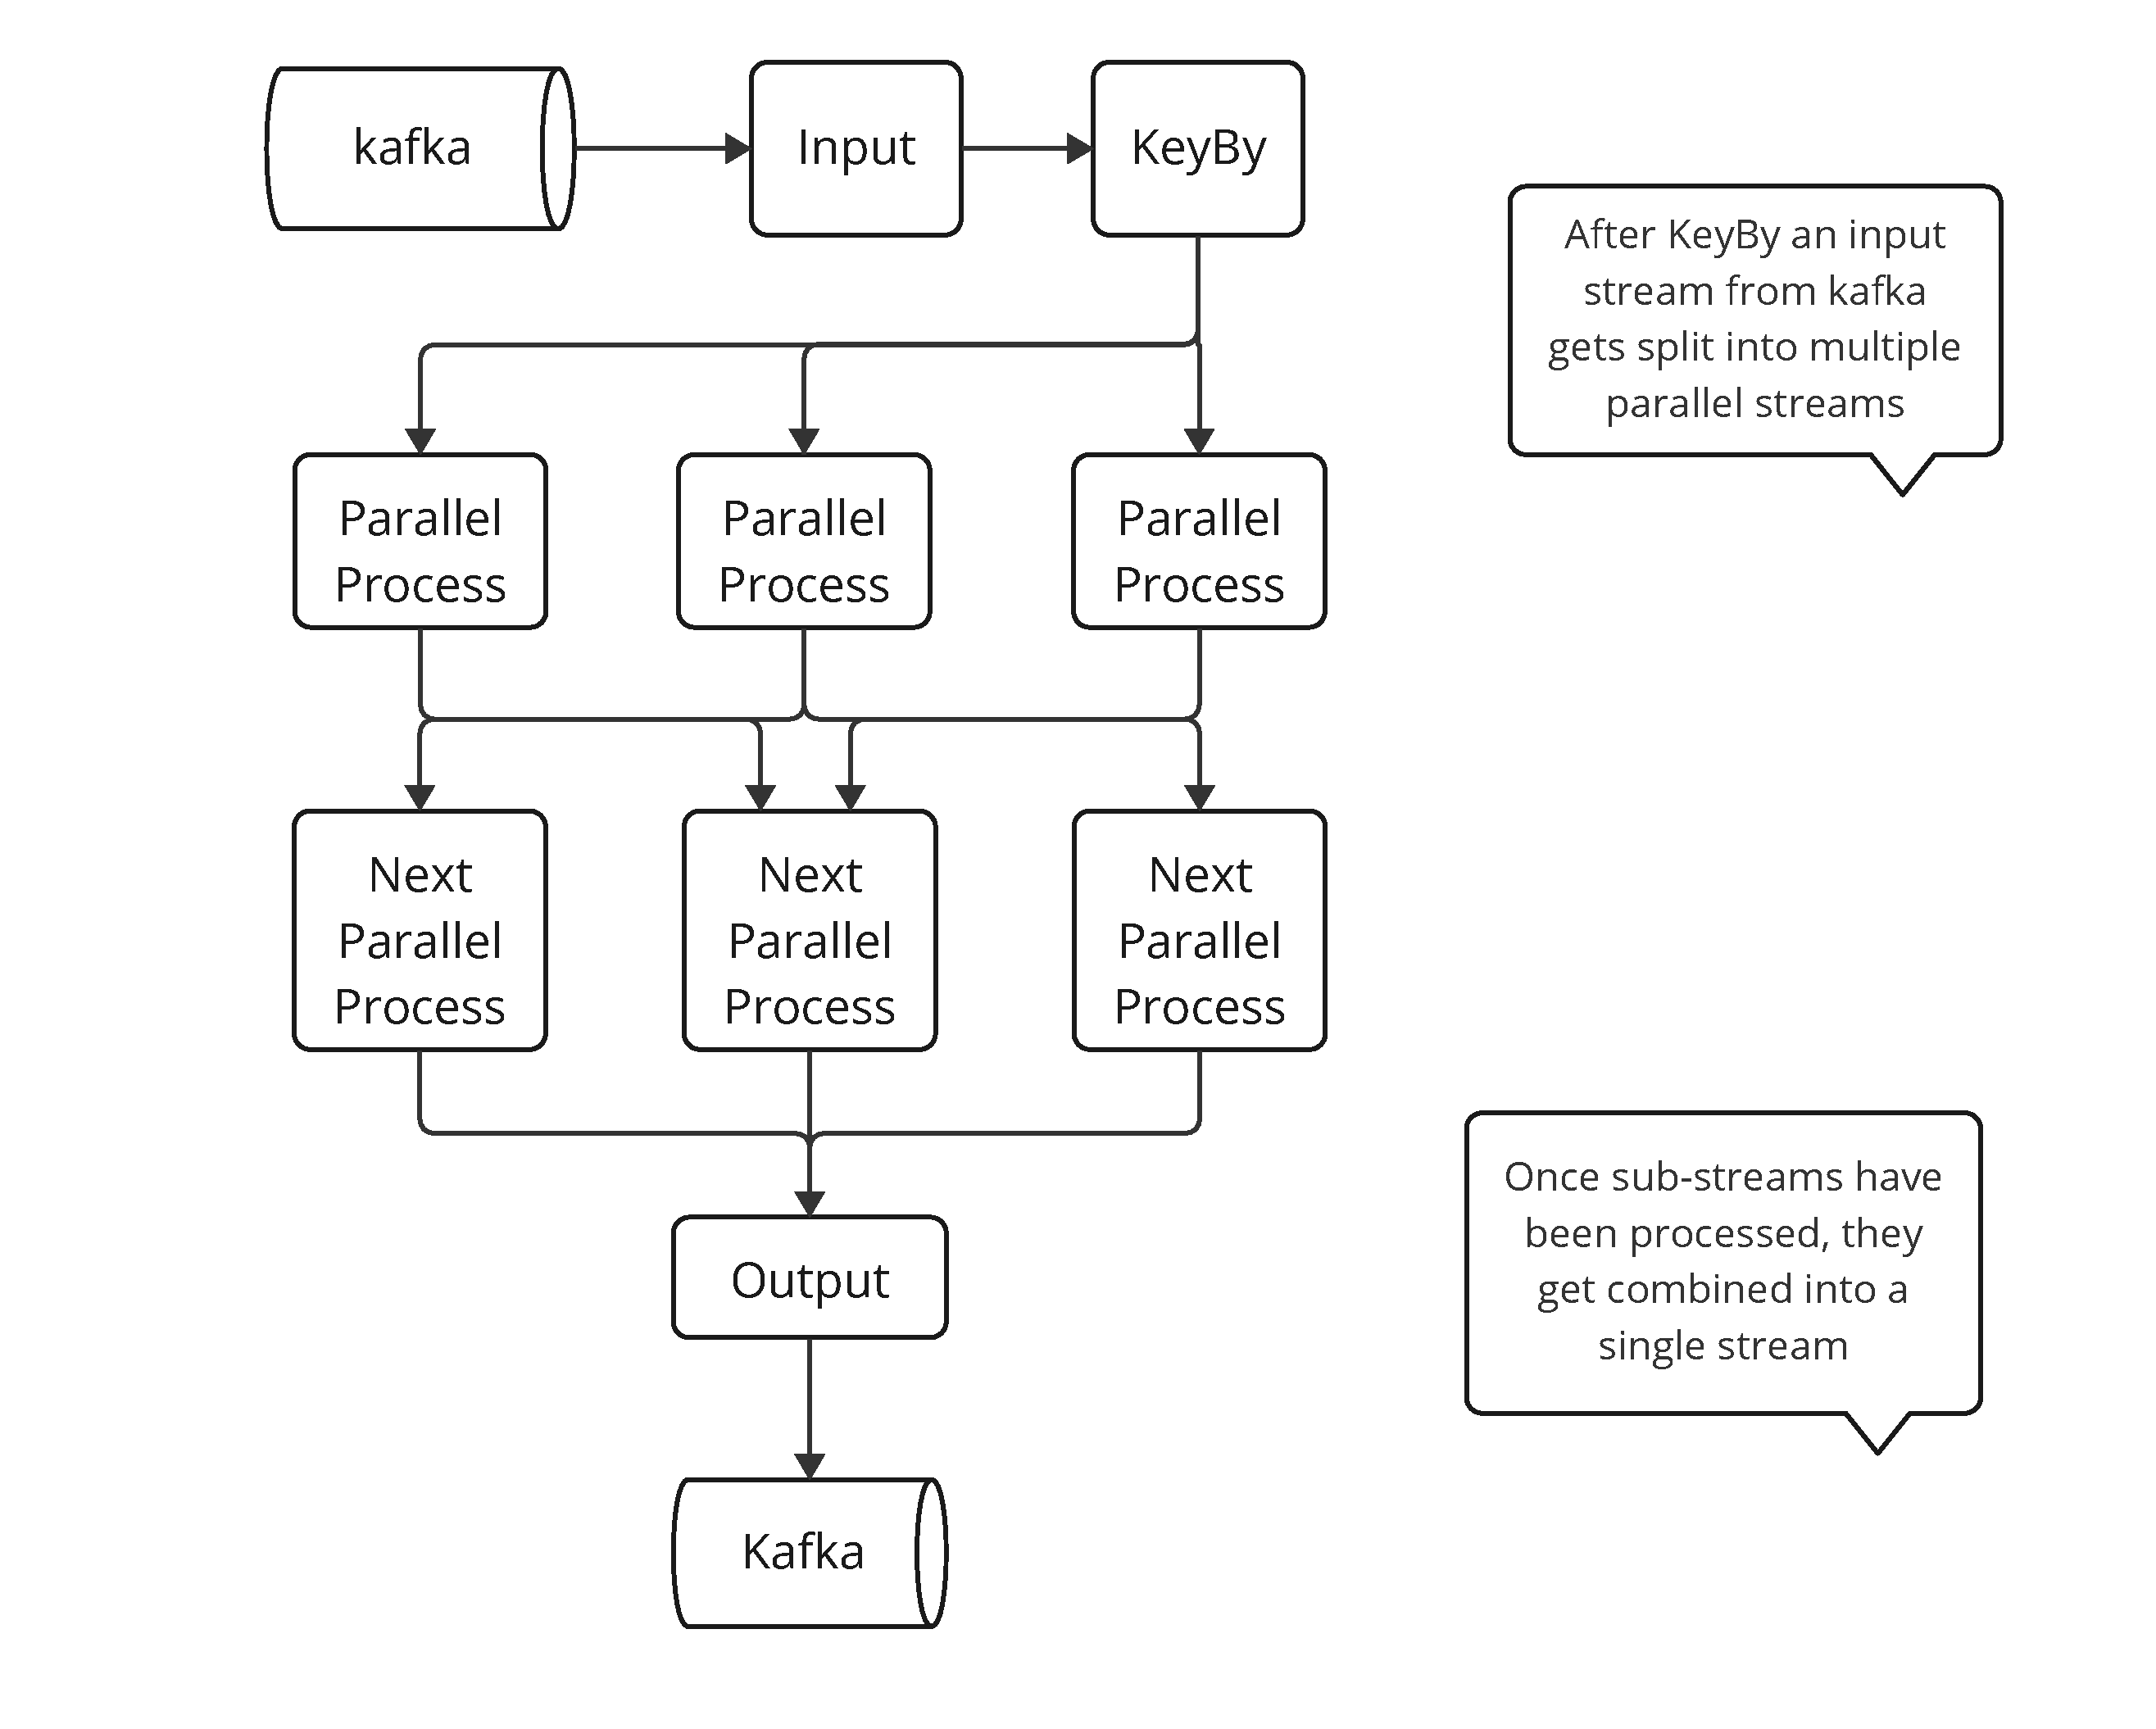
\includegraphics[width=1\textwidth]{figures/dataflow-graph}
%    \caption{\textit{An example of data stream execution with dataflow graphs.}}
%    \label{fig:dataflow-graph}
%\end{figure}
%
%\newpage

%\subsection{Data Parallelism and Task Parallelism}\label{subsec:data-parallelism-and-task-parallelism}
%Data parallelism and task parallelism might sound confusing even for experienced developers.
%In dataflow graphs, parallelism can be achieved in two ways.
%Data parallelism with partitioning input data and executing tasks of
%the same operation on data subsets in parallel, allowing for efficient processing
%of large data volumes and spreading the computation load across multiple computing nodes.
%Task parallelism, on the other hand, refers to tasks from different operators
%performing computations on the same or different data in parallel,
%which enables better utilization of the computing resources in a cluster.
%
%\begin{figure}[H]
%    \centering
%    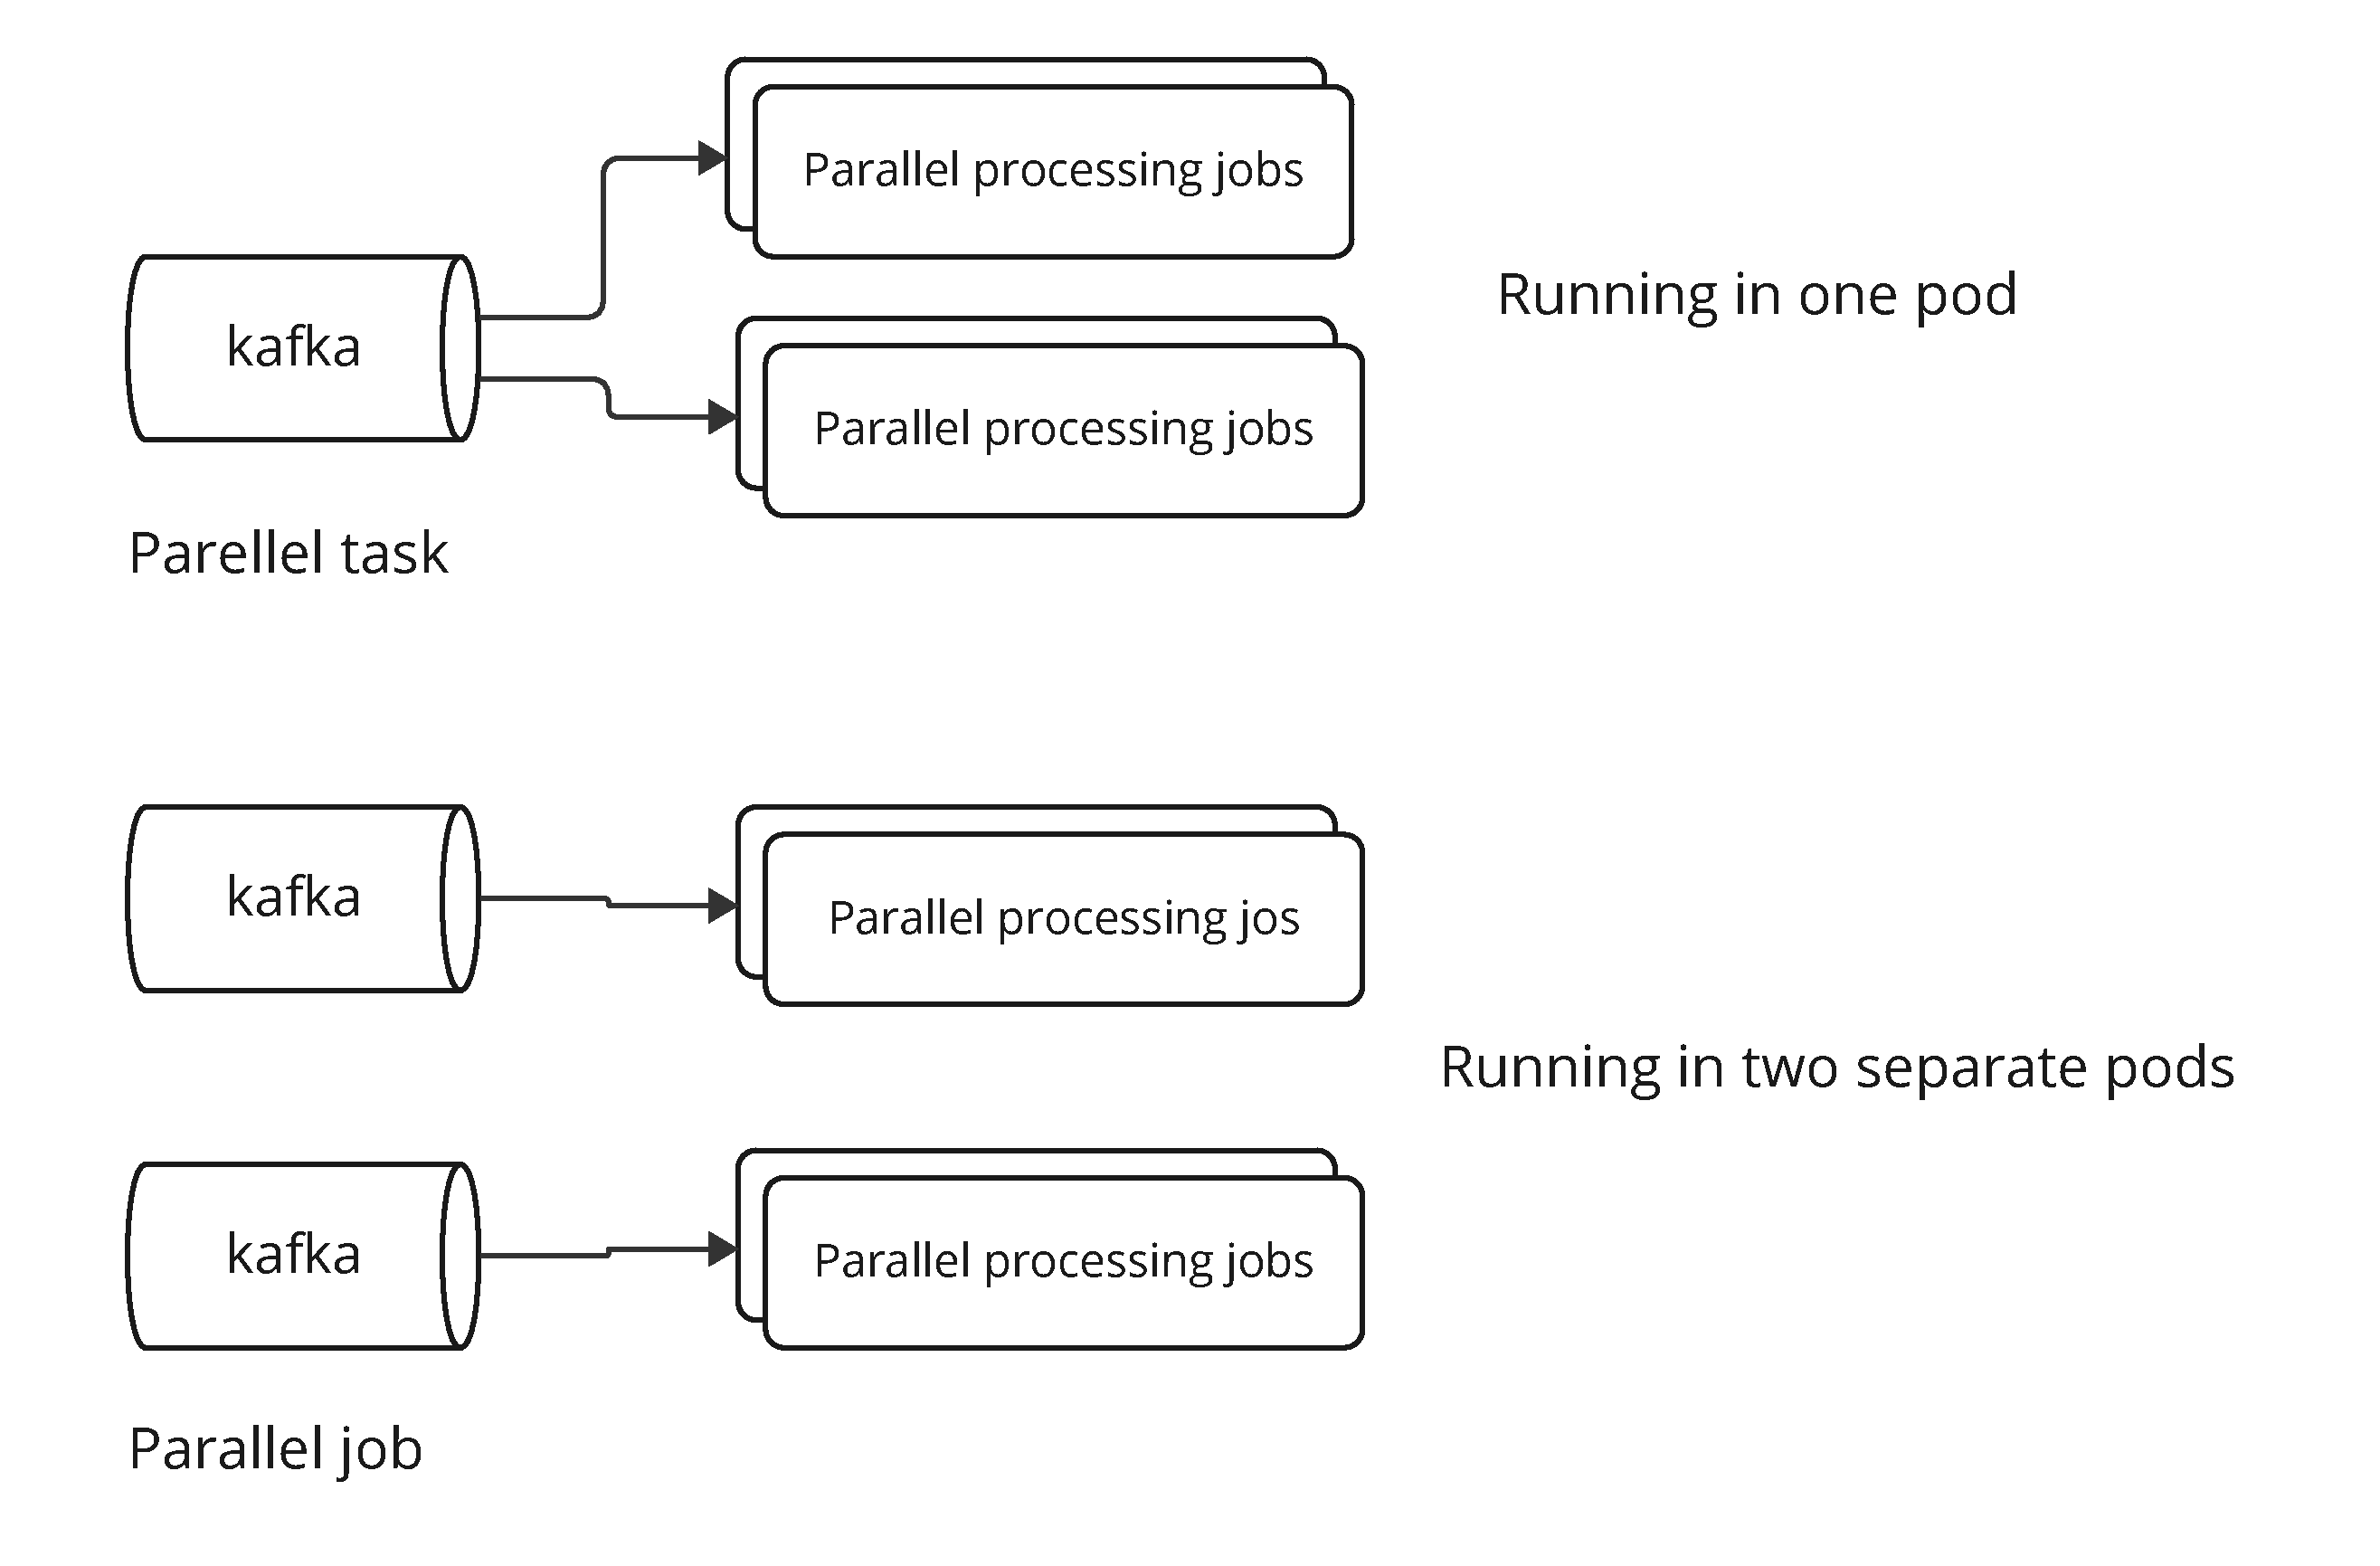
\includegraphics[width=1\textwidth]{figures/parallel-jobs}
%    \caption{\textit{An example of data stream execution with dataflow graphs.}}
%    \label{fig:parallel-job}
%\end{figure}
%
%In order to get better understanding, Figure \ref{fig:parallel-job} depicts a visual difference.
%Job parallelism defined how many parallel task are running in separate execution node,
%but performing as one single app.
%In case of Kafka, each job's task processes a subset of kafka partitions, such
%that all tasks process all partitions.
%Kafka knows how to spread partitions among all tasks, a developer
%don't need to worry about it, only if there's a very specific case for that.
%In general partitioning should work automatically, the only a number of partitions
%is under developer's responsibility.
%There's a formula which defined a number of partition for a project which is getting started,
%but as a data volumes grow it's good practice to add more partitions manually.
%Moder monitoring tools help to identify such moment, when a number of partitions
%should increase to handle new data volumes.
%
%\subsection{Data Exchange Strategies}\label{subsec:data-exchange-strategies}
%
%\begin{description}
%    \item[Forwarding] The forwarding approach passes data straight from one task
%    to the downstream task without reshuffling or rearrangement.
%    The downstream operator processes data in the same sequence and partitioning
%    as the upstream operator.
%    Forwarding is the most efficient strategy, due to less overhead and network communication.
%    \item[Partitioning] Data is redistributed among parallel jobs depending on a key or function.
%    Key-based partitioning, which shuffles and groups data by key values, is the most frequent.
%    Keyed aggregations, joins, and groupBy use this method.
%    Partitioning processes all records with the same key.
%    \item[Broadcast] Data from upstream jobs is replicated and delivered to downstream activities.
%    In a broadcast join or when a small dataset needs to be available to all downstream
%    for processing, then broadcast strategy is used.
%    \item[All-to-All] The all-to-all technique sends all upstream records to all downstream jobs.
%    This method is utilized when data order or partitioning doesn't matter
%    or when every task must process the complete dataset.
%    For large datasets, this method has a substantial transmission overhead.
%    \item[Rebalancing] Rebalancing redistributes data evenly across downstream processes.
%    It prevents data skew and load imbalance from uneven data distribution.
%    Rebalancing guarantees that downstream tasks receive roughly the same quantity of records,
%    improving performance and resource use.
%    \item[Random] Random uniform distribution across downstream tasks.
%\end{description}
%
%
%\begin{figure}[H]
%    \centering
%    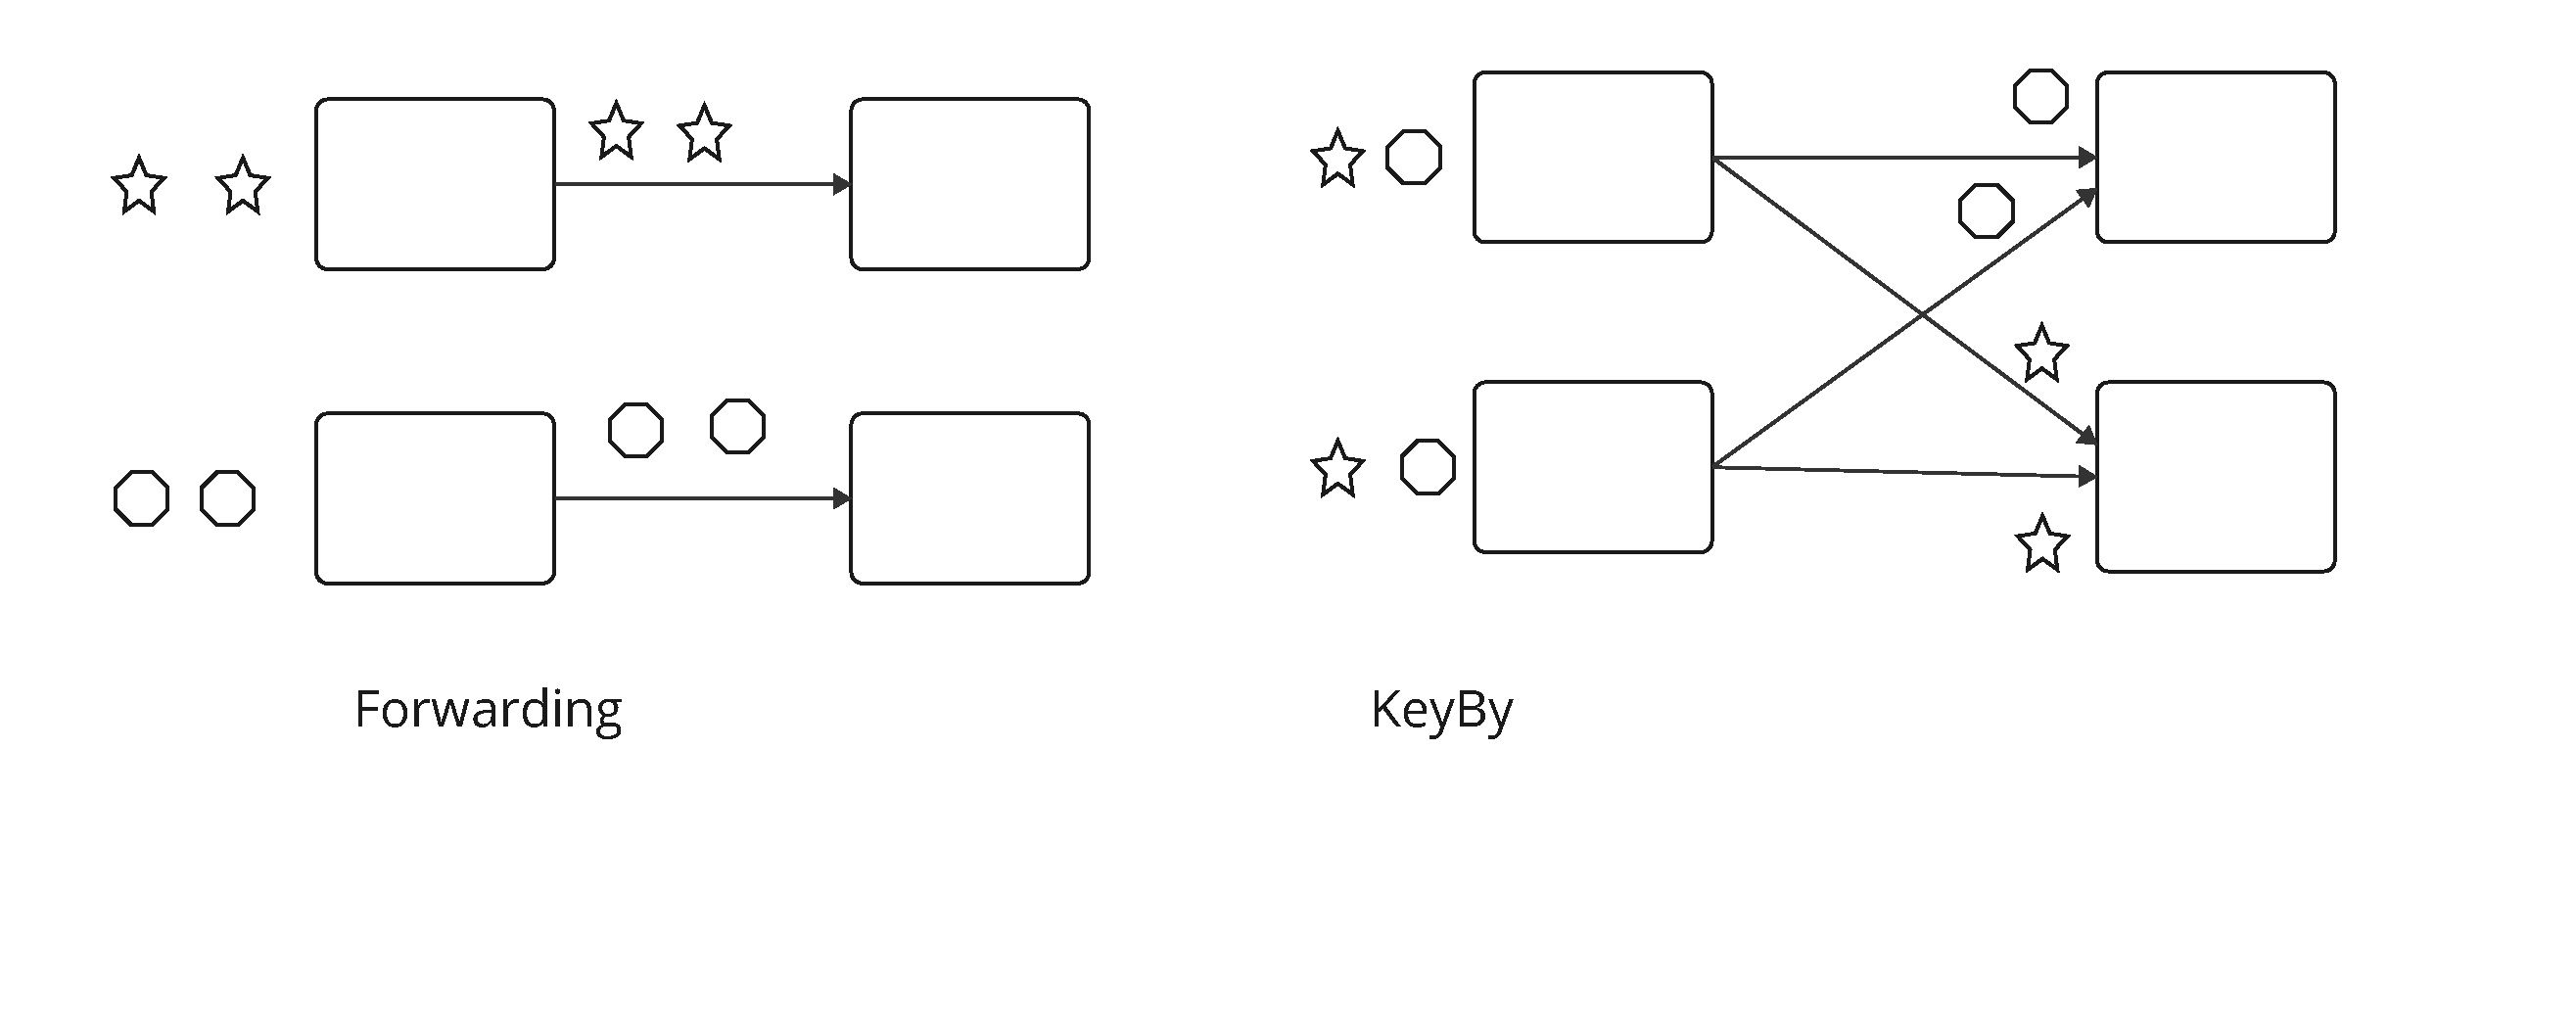
\includegraphics[width=1\textwidth]{figures/forward}
%    \caption{\textit{An example of forwarding and partitioning by key.}}
%    \label{fig:forward}
%\end{figure}

\newpage
\section{Stream Processing Challenges}\label{sec:-challanges}
Since this research is focusing on stateful streaming,
a variety of challenges must be handled by a new solution.
Detailed challenges are described in \cite{spark_structured_streaming}.

\begin{description}
    \item[State Management] In stateful stream processing systems, a state represents a unit of information stored, accessed, and updated by a key. The simplest example of a key-based state is a counter. Setting up state storage in distributed systems is challenging due to different state sizes, update frequencies, and storage types. Stream processing frameworks must ensure consistency and minimal latency while managing state across multiple workers. Frameworks come with built-in state backends and metrics exporters that expose information about the system performance.
    Example of state metrics: represent state size, memory usage, latency, and read-write metrics.
    \item[Fault tolerance] It includes snapshot configurations, message commit time interval, storage configurations,
    state monitoring.
    \item[Scalability] Since the load in data-intensive production systems may vary over time,
    it's crucial to design the system as auto-scalable.
    Auto-scalable systems automatically adjust the number of workers needed for incoming data in real-time.
    Having redundant workers might lead to additional expenses, while insufficient
    worker replicas lead to system crashes and slowness..
    \item[Rebalancing] Repartition is a core feature that deals with fault tolerance
    and scalability in case of fault.
    It's part of the rebalancing process.
    The controller coordinator is responsible for repartition if a consumer is no longer responsive.
    An example is Kafka's consumer group \cite{kafka2020}.
    \item [Processing latency] Apache Flink and Kafka Stream are able
    to handle a load in a reasonable time range, but might have different latency in case of stateful stream processing
    with different state sizes and input throughout.
    An example of such benchamarks \cite{Henning_2024}.
    \item[Delivery guarantee] The Most common types of semantics in stream processing are at least once semantics, and
    exactly once semantics that deal with a complex commit process.
    These processes are described here \cite{confluentExactlyOnce, flinkExactlyOnce2018}.
    \item[Deployment] At this time, streaming frameworks have already Kubernetes
    integration which allows managing deployment and resources.
    However, complex cloud configurations require deep expertise.
\end{description}


\section{Directed Acyclic Graph Model in Stream Processing}\label{subsec:dataflow-graph}

\begin{figure}[H]
    \centering
    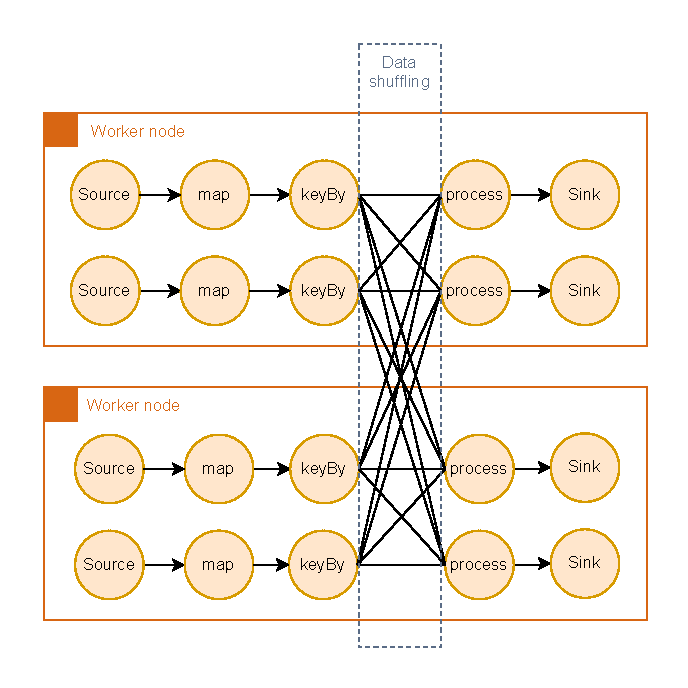
\includegraphics[width=1\textwidth]{figures/data-shuffling}
    \caption{\textit{This diagram illustrates how data flows from Source to Sink
        passing through various shuffling and processing stages using directed acyclic graphs.
    The most popular frameworks that use DAG model are: Kafka Streams, Apache Flink, Apache Spark, Hazelcast Jet, Apache Storm.}}
    \label{fig:data-shuffling}
\end{figure}

In big data and real-time stream processing frameworks, processing and analyzing data as it flows through systems is crucial. Data streaming frameworks have emerged as powerful tools to handle such tasks,
and at the heart of these frameworks lies a fundamental concept: the Directed Acyclic Graph (DAG) \cite{flinkCheckpoints, Dataflow2015, flink_dag, kafka_streams_topology}.
DAG model is illustrated on Figure \ref{fig:data-shuffling}.
Stream processing based on DAG consists of the following components \cite{kafka_streams_topology, kleppmann2017, spark_structured_streaming}.

\begin{description}
    \item[Source] A source is the component in a data streaming framework that ingests partitioned streams of data from external systems,
    initiating the data processing pipeline.
    \item[map] A map is a data transformation component that applies a specified function to each element in the input data stream, producing a transformed output stream.
    It is commonly used to transform data records from one form to another as they pass through the processing pipeline.
    \item[keyBy] A keyBy component in a data streaming framework shuffles and partitions the data stream based on a key extracted from each data record,
    ensuring that records with the same key are sent to the same downstream task for processing.
    \item[process] A process component in a data streaming framework is responsible for stateful processing, maintaining and
    updating the state as it processes each data record.
    This allows for complex event processing and aggregation based on the changing state.
    \item[Sink] A sink is the component in a data streaming framework that sends processed and
    partitioned data records to an external system for storage, analysis, or further processing.
    \item[Data shuffling] Data shuffling between the keyBy and process components in a data streaming framework
    involves redistributing the data across different partitions or nodes based on the key extracted from each data record.
    This is a crucial step for ensuring that records with the same key are processed together,
    enabling stateful operations and accurate aggregation.
\end{description}


\newpage
\section{Kafka Cluster}\label{sec:kafka-as-a-data-provider:-challenges}
The use case in this research uses Kafka cluster of 3 brokers as a
data source and data sink.
Kafka cluster plays a crucial role in evaluation fault tolerance performance
since both Apache Flink and Kafka Streams based prototypes represent a
cluster of one Kafka consumer group.

\begin{figure}[H]
    \centering
    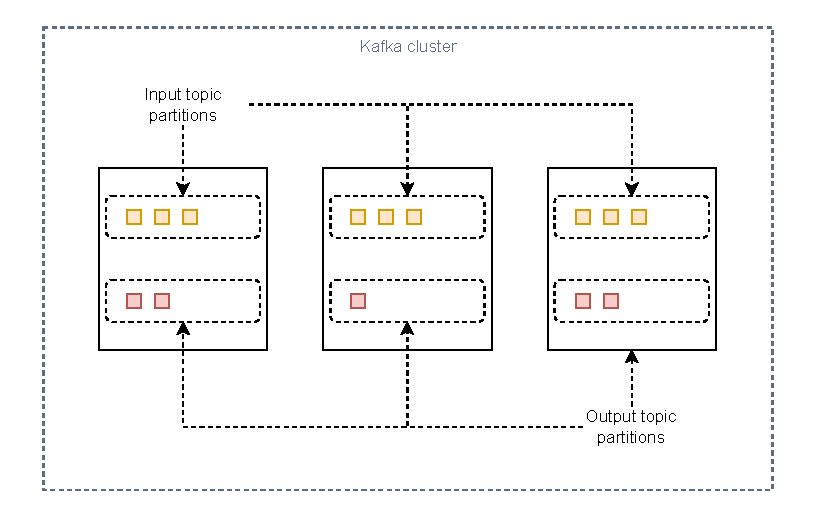
\includegraphics[width=1\textwidth]{figures/kafka-cluster}
    \caption{\textit{Illustration of simplified Kafka cluster model that is uses in this case study.
    In the case study the cluster consists of 3 brokers and 2 topics with 50 partitions for each topic.}}
    \label{fig:producer}
\end{figure}

While the model in Figure \ref{fig:producer} illustrates a simple diagram, a real Kafka cluster is composed of advanced
components such as leader election, a control plane for cluster management,
and robust mechanisms for data replication and fault tolerance.
This case study does not evaluate the fault tolerance of the Kafka cluster,
but it highlights Kafka's extensive use as a core component for data processing.
The Full description of Kafka cluster leader election and control is
described in the official Kafka documentation \cite{confluentControlPlane}.
Down below are the core components of the Kafka cluster that are described in details \cite{kafka2020}.

\begin{description}
    \item[Kafka Consumer Group] A Kafka consumer group is a collection of consumers that work together to
    read records from one or more Kafka topics.
    Each consumer in the group reads data from a different subset of the partitions,
    allowing for parallel processing and load balancing.
    \item[Kafka Consumer] A Kafka consumer is a client application that subscribes to one
    or more Kafka topics and processes the data records published to those topics.
    Consumers read data in real-time and can be part of a
    consumer group for distributed processing.
    \item[Kafka Producer] A Kafka producer is a client application that publishes
    data records to Kafka topics. Producers send records to specific topics and can partition
    data across multiple partitions within those topics for scalability and load balancing.
    \item[Kafka Broker] A Kafka broker is a server that hosts Kafka topics and manages
    the storage, retrieval, and replication of data records.
    Brokers handle the incoming data from producers, serve data to consumers, and ensure data durability and fault tolerance through replication.
    \item[Leader Election] Leader election in Kafka is the process by
    which one broker is designated as the leader for each partition.
    The leader is responsible for all reads and writes for the partition,
    ensuring consistent and orderly data management.
    Other brokers that store replicas of the partition data act as followers.
\end{description}


\section{State Recovery}\label{subsec:state-recovery}
State recovery is crucial in distributed stream processing systems to ensure fault tolerance and consistency.
When a system encounters failures, it must recover its state and resume processing without data loss or inconsistency.
This section delves into the state recovery mechanisms that are used in Apache Flink and Kafka Streams,
focusing on distributed snapshots and change logs.

\subsection{Distributed Snapshots}\label{subsec:distributed-snapshots}
Distributed snapshots are essential for capturing a consistent global state of a distributed system.
The Chandy-Lamport algorithm, introduced by K. Mani Chandy and Leslie Lamport in their 1985 paper
\("\)Distributed Snapshots: Determining Global States of a Distributed System,\("\) provides a robust method to achieve
this \cite{chandy1985distributed}.
Distributed snapshots are foundational in stream processing frameworks like Apache Flink,
enabling them to maintain accurate states across distributed
nodes by consistent state recovery and fault tolerance.
Later, the ideas behind the Chandy-Lamport algorithm were used to implement Asynchronous Barrier Snapshotting \cite{flinkCheckpoints}
algorithm for Apache Flink.
ABS algorithms quarantine consistence snapshots and are especially efficient in case of
frequent snapshotting starting from 2 seconds period.
These benchmarks are provided in \cite{flinkCheckpoints}.
Since the case study uses Kafka as a data source, snapshots keep track of the latest committed message to ensure state consistency.
This allows for rerunning state updates by processing uncommitted Kafka records during recovery.


\begin{figure}[H]
    \centering
    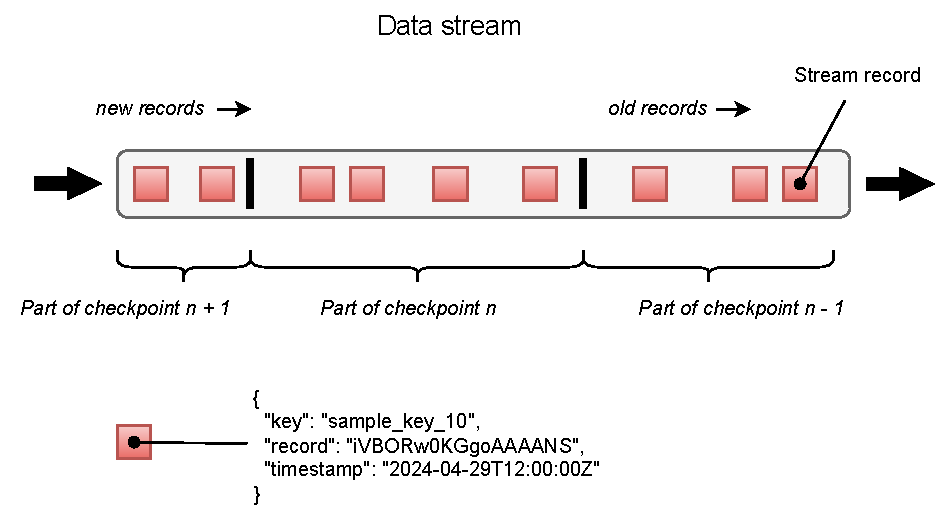
\includegraphics[width=1\textwidth]{figures/data-stream}
    \caption{\textit{Illustration of snapshots applied for data stream.}}
    \label{fig:flink-stream-snapshots}
\end{figure}


Simplified stream snapshotting period is illustrated on Figure \ref{fig:flink-stream-snapshots}.
The ABS algorithm performs asynchronous micro-pauses to capture
records currently being processed by a worker.
This ensures a proper snapshot is taken and saved in the configured storage,
maintaining data consistency and enabling efficient state recovery.
The storage and snapshot interval for the case study is illustrated on Figure \ref{fig:flink-snapshots}.

\begin{figure}[H]
    \centering
    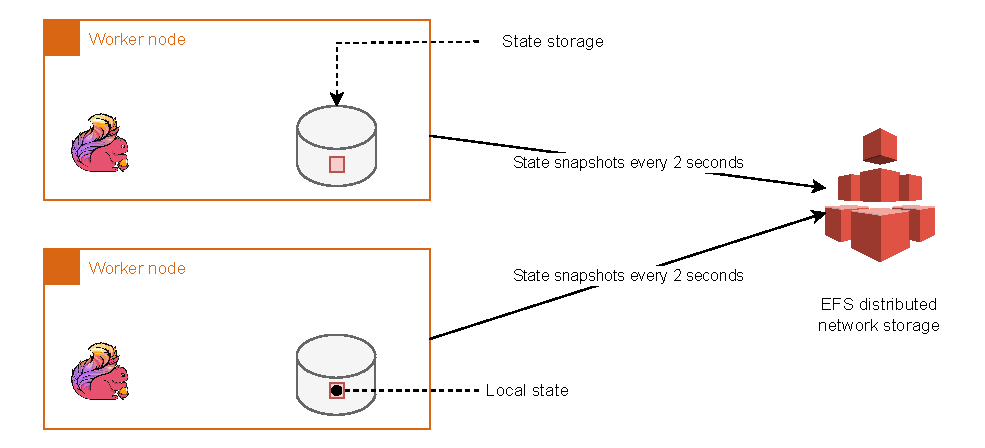
\includegraphics[width=1\textwidth]{figures/flink-snapshots}
    \caption{\textit{Illustration of snapshots for an Apache Flink-based prototype in this case study.
    Snapshots get stored to AWS EFS network storage.}}
    \label{fig:flink-snapshots}
\end{figure}



\subsection{Change Logs}\label{subsec:change-logs}
In Kafka Streams, state stores are used to keep track of accumulated state, such as counts, sums, or other aggregations.
These state stores are backed by change logs, which are special Kafka topics that record every update to the state store \cite{kafka_streams_intro}.

\begin{figure}[H]
    \centering
    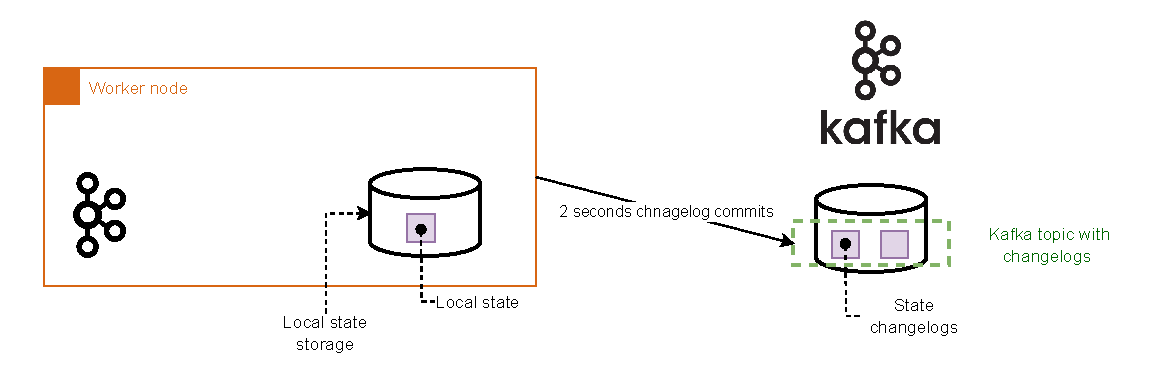
\includegraphics[width=1\textwidth]{figures/kafka-changelogs}
    \caption{\textit{Illustration of changelogs for Kafka Streams-based prototype in this case study.
    Changelogs get stored to Kafka cluster.}}
    \label{fig:kafka-snapshots}
\end{figure}

Illustration on Figure \ref{fig:kafka-snapshots} demonstrates Kafka Streams
stage management model.
Change log topics record every update to the state store.
It includes any inserts, updates, or deletes within the state store.
Each state change is logged as a new record in the change log topic.
If the application crashes, it can replay the change log topic from the beginning to reconstruct
the state store with all user sessions up to the point of the crash.
By capturing every state update as an ordered log of key-value pairs,
Kafka Streams algorithms ensure that stateful stream processing applications can recover
from failures and continue processing without data loss.
Using 2 seconds commit interval makes the case study comparison more accurate since
Apache Flink based prototype uses 2 seconds snapshot interval.

\section{Rule Based Matching Service}\label{sec:rule-based-matching-service}
The core component of prototypes in this case study is the rule based matching service.
The goal of such a service is an emulation of rules based logs matchers.
Each rule represents a logical consumer that has a certain propability matching with
an incoming data record.
The core component of prototypes in this case study is the rule-based matching service.
The goal of such a service is to emulate rule-based log matches.
Each rule represents a logical consumer with a specific matching probability
with an incoming data record.


\begin{figure}[H]
    \centering
    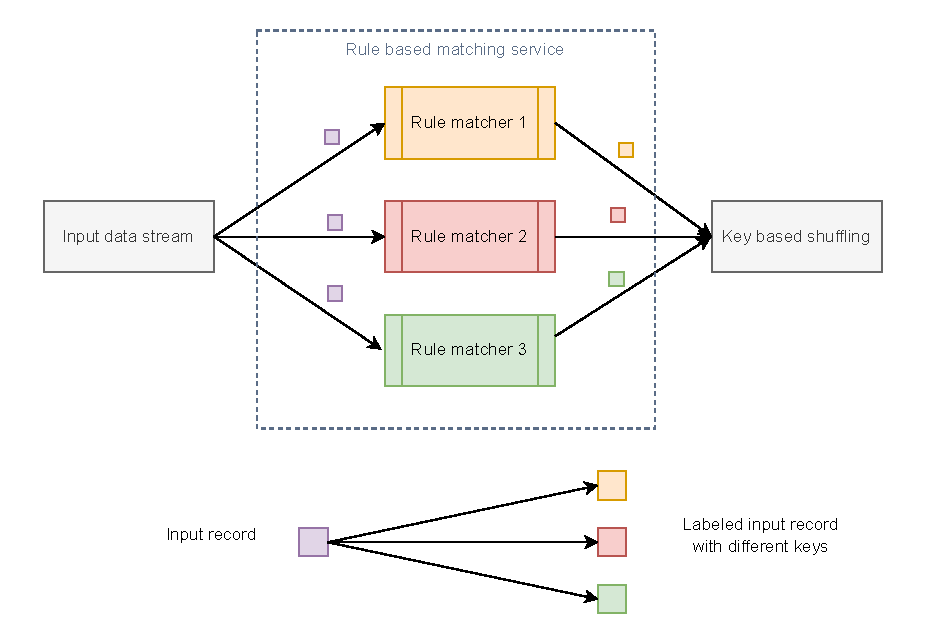
\includegraphics[width=1\textwidth]{figures/rule-matcher}
    \caption{\textit{Illustration of the rule based matching service.}}
    \label{fig:rule-matcher}
\end{figure}

Rule-based matcher in illustrated on Figure \ref{fig:rule-matcher}.
Each incoming record is processed through all the rule matchers. For each match, a new keyed record is generated,
where the key represents the record's label.
All rule matchers have a fixed matching probability in this use case simulation.
For example, if there are 10 rules and the matching probability is 0.1,
then it is expected that at least 1 rule will match per record,
resulting in at least one labeled record for further shuffling and processing.
If the matching probability is 1, then 10 labeled records get shuffled and processed for 1 incoming record.
All rule matchers are based on the seed that guarantees experiment replication.
The real use case might be implemented with Intel Hyperscan (see Figure \cite{intelHyperscan}),
but this case study does not focus on that.
